\def\difficulty{1}
\sujet{Image Filtering using PDEs}
\index{Filtering!Partial Differential Equations}

\begin{note}This tutorial aims to process images with the help of partial differential equations.\end{note}

\noindent The different processes will be applied on the following MR image Fig. \ref{fig:pde:enonce:irm}.

\begin{figure}[htbp]
\centering
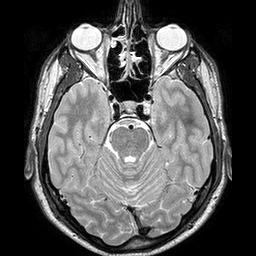
\includegraphics[width=5cm]{cerveau.jpg}
\caption{MRI image of a human brain.}
\label{fig:pde:enonce:irm}
\end{figure}

\section*{Notations}
The different operators used here are:
\begin{eqnarray}
 \vec{A} = \left( \begin{array}{c}
                   A_x \\
                   A_y 
                  \end{array}
\right)
\end{eqnarray}

\begin{eqnarray}\divergence \overrightarrow{A} = \frac{\partial A_x}{\partial x} + \frac{\partial A_y}{\partial y}
\end{eqnarray}


\begin{eqnarray}
\vec{\grad}\,u(x,y) =\nabla u= \left( \begin{array}{c}
                       \frac{\partial u}{\partial x} \\
                       \frac{\partial y}{\partial y}
                      \end{array}
\right)
\end{eqnarray}
The Laplacian operator is denoted $\Delta u=\nabla^2 u= \divergence \overrightarrow{\grad}\,u$. A numerical approximation can be used, but is not recommanded in this tutorial.

\section{Linear diffusion}
\index{Filtering!Linear Diffusion}
\index{Heat Equation}
The heat equation is defined as follows:
\begin{eqnarray}
\left\{\begin{array}{ccl}
\displaystyle\frac{\partial u}{\partial t}(x,y,t)&=&\divergence (\nabla u(x,y,t))\\
&=&\displaystyle\frac{\partial^2 u}{\partial x^2}(x,y,t)+\displaystyle\frac{\partial^2 u}{\partial y^2}(x,y,t)\\
u(x,y,0)&=&f(x,y)
\end{array}
\right.
\end{eqnarray}
If $f(x,y)$ is an image (with $(x,y)\in D\subset\mathbb{R}^2$, $D$ is the spatial support), this defines a filtering method that is equivalent to the convolution of $f$ by a Gaussian function \cite{Koenderink1984}.
This equation can be solved by a finite difference numerical method.

\subsection{Numerical scheme}
The following notations are employed. $N$, $S$, $E$, $W$ stand for north, south, east and west.
\begin{eqnarray}
\begin{array}{ll}
 +\delta^N u &= \frac{u(x,y+h)-u(x,y)}{h} \\
 -\delta^S u &= \frac{u(x,y-h)-u(x,y)}{h} \\
 -\delta^E u &= \frac{u(x-h,y)-u(x,y)}{h} \\
 +\delta^W u &= \frac{u(x+h,y)-u(x,y)}{h}  
 \end{array}
\end{eqnarray}

Thus, the numerical scheme is ($h$ has value 1):
\begin{align}
 \frac{u^{t+1}-u^t}{\delta t} &= \frac{1}{h}\left\{\delta^N u - \delta^S u + \delta^E u - \delta^W u\right\}
\end{align}

\begin{qbox}
\begin{enumerate}
	\item Code the numerical scheme. It should use two parameters: the number of iterations $n$, and the step time $\delta t$.
	\item Filter the original image by varying the parameters of the discrete diffusion process.
	\item Comment the filtering results. Compare the results with the Gaussian filter.
\end{enumerate}
\end{qbox}


\section{Nonlinear diffusion}
\index{Filtering!Non Linear Diffusion}
Image filtering by nonlinear diffusion reduces noise in a controled way. The diffusion coefficient is locally adapted, becoming negligible as object boundaries are approached.\\
The heat equation is replaced by the following PDE:
\begin{eqnarray}
\left\{\begin{array}{ccl}
\displaystyle \frac{\partial u}{\partial t}(x,y,t)&=&\divergence\left(c(\|\nabla u(x,y,t)\|)\cdot\nabla u(x,y,t)\right)\\
u(x,y,0)&=&f(x,y)
\end{array}
\right.
\end{eqnarray}
with $c$ the diffusion fonction satisfying the following properties:
\begin{itemize}
	\item $c(0)=1$,
	\item $\displaystyle \lim_{s\rightarrow +\infty}sc(s)=0$,
	\item $\forall s>0, c'(s)\leq 0$.
\end{itemize}

\noindent Perona and Malik have proposed 2 diffusion coefficients \cite{Perona1990,Catte1992}:
\begin{itemize}
	\item $c_1$ : $\displaystyle \exp\left(-\left(\displaystyle\frac{s}{\alpha}\right)^2\right)$,
	\item $c_2$ : $\displaystyle \frac{1}{1+\left(\displaystyle\frac{s}{\alpha}\right)^2}$.
\end{itemize}

\subsection{Numerical scheme}
The numerical scheme is the following:
\begin{align}\frac{u^{t+1}-u^t}{\delta t} &= \frac{1}{h^2}\left\{ c(|\delta^N u|)\cdot \delta^N u + c(|\delta^S u|)\cdot \delta^S u \right. \\
            &\hspace*{2cm} \left. + c(|\delta^E u|)\cdot \delta^E u + c(|\delta^W u|)\cdot \delta^W u \right\}\nonumber
\end{align}
\begin{qbox}

\begin{enumerate}
	\item Code the numerical scheme
	\item Filter the original image by varying the parameters of the discrete nonlinear diffusion process.
	\item Comment and compare the filtering results with the previous scheme.
\end{enumerate}
\end{qbox}

\section{Degenerate diffusion}
\index{Filtering!Degenerate Diffusion}
The following degenerate PDEs have been shown to be equivalent to the morphological operators of dilation and erosion (using a disk as structuring element, see tutorial on mathematical morphology):\vspace*{-5pt}
\begin{eqnarray}
\left\{\begin{array}{ccl}
\displaystyle \frac{\partial u}{\partial t}(x,y,t)&=&+\|\nabla u(x,y,t)\|\\
u(x,y,0)&=&f(x,y)
\end{array}
\right.\\
\left\{\begin{array}{ccl}
\displaystyle \frac{\partial u}{\partial t}(x,y,t)&=&-\|\nabla u(x,y,t)\|\\
u(x,y,0)&=&f(x,y)
\end{array}
\right.
\end{eqnarray}

\subsection{Numerical schemes}
The previous numerical scheme is easy to find, but the results present large differences with the dilation and erosion operators (shocks due to discontinuities in the original image). This is why the following numerical scheme is preferred \cite{Maragos1996}:

For the erosion:\vspace*{-5pt}
\begin{align}\frac{u^{t+1}-u^t}{\delta t} = \frac{1}{h^2}
\sqrt{\begin{aligned}&max^2(0,-\delta^N u) + min^2(0,-\delta^S u) \dots\\
&\hspace{1cm}+ max^2(0,-\delta^W u) + min^2(0,-\delta^E u)
\end{aligned}
}
\end{align}

For the dilation:\vspace*{-5pt}
\begin{align}\frac{u^{t+1}-u^t}{\delta t} = \frac{1}{h^2}\sqrt{\begin{aligned}&min^2(0,-\delta^N u) + max^2(0,-\delta^S u) \dots\\
&\hspace{1cm}+ min^2(0,-\delta^W u) + max^2(0,-\delta^E u)
\end{aligned}                                                                 
}
\end{align}

\begin{qbox}
\begin{enumerate}
	\item Code the numerical scheme.
	\item Filter the original image while varying the parameters of the discrete degenerate diffusion process.
	\item Comment the morphological filtering results and compare the nu\-me\-ri\-cal sche\-me to the ap\-proach with operational windows.
\end{enumerate}
\end{qbox}

